% Created by tikzDevice version 0.12 on 2019-01-19 16:45:08
% !TEX encoding = UTF-8 Unicode
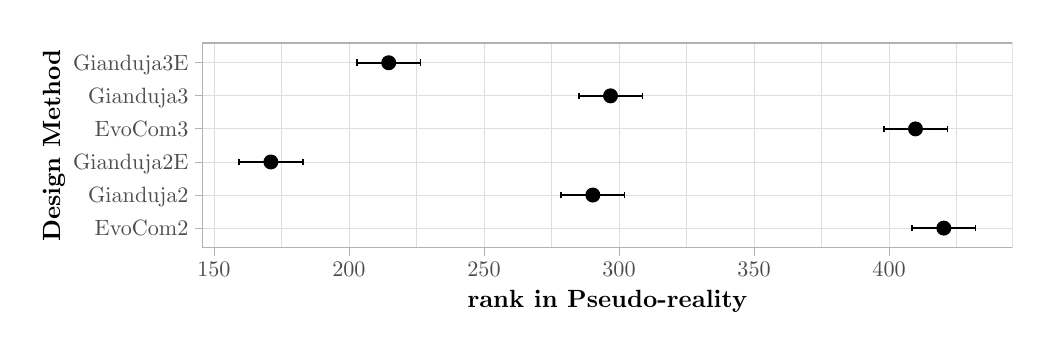
\begin{tikzpicture}[x=1pt,y=1pt]
\definecolor{fillColor}{RGB}{255,255,255}
\path[use as bounding box,fill=fillColor,fill opacity=0.00] (0,0) rectangle (361.35,108.41);
\begin{scope}
\path[clip] (  0.00,  0.00) rectangle (361.35,108.40);
\definecolor{drawColor}{RGB}{255,255,255}
\definecolor{fillColor}{RGB}{255,255,255}

\path[draw=drawColor,line width= 0.6pt,line join=round,line cap=round,fill=fillColor] (  0.00,  0.00) rectangle (361.35,108.40);
\end{scope}
\begin{scope}
\path[clip] ( 63.07, 28.81) rectangle (355.85,102.90);
\definecolor{fillColor}{RGB}{255,255,255}

\path[fill=fillColor] ( 63.07, 28.81) rectangle (355.85,102.90);
\definecolor{drawColor}{gray}{0.87}

\path[draw=drawColor,line width= 0.1pt,line join=round] ( 91.69, 28.81) --
	( 91.69,102.90);

\path[draw=drawColor,line width= 0.1pt,line join=round] (140.49, 28.81) --
	(140.49,102.90);

\path[draw=drawColor,line width= 0.1pt,line join=round] (189.28, 28.81) --
	(189.28,102.90);

\path[draw=drawColor,line width= 0.1pt,line join=round] (238.08, 28.81) --
	(238.08,102.90);

\path[draw=drawColor,line width= 0.1pt,line join=round] (286.87, 28.81) --
	(286.87,102.90);

\path[draw=drawColor,line width= 0.1pt,line join=round] (335.67, 28.81) --
	(335.67,102.90);

\path[draw=drawColor,line width= 0.3pt,line join=round] ( 63.07, 35.98) --
	(355.85, 35.98);

\path[draw=drawColor,line width= 0.3pt,line join=round] ( 63.07, 47.93) --
	(355.85, 47.93);

\path[draw=drawColor,line width= 0.3pt,line join=round] ( 63.07, 59.88) --
	(355.85, 59.88);

\path[draw=drawColor,line width= 0.3pt,line join=round] ( 63.07, 71.83) --
	(355.85, 71.83);

\path[draw=drawColor,line width= 0.3pt,line join=round] ( 63.07, 83.78) --
	(355.85, 83.78);

\path[draw=drawColor,line width= 0.3pt,line join=round] ( 63.07, 95.73) --
	(355.85, 95.73);

\path[draw=drawColor,line width= 0.3pt,line join=round] ( 67.30, 28.81) --
	( 67.30,102.90);

\path[draw=drawColor,line width= 0.3pt,line join=round] (116.09, 28.81) --
	(116.09,102.90);

\path[draw=drawColor,line width= 0.3pt,line join=round] (164.89, 28.81) --
	(164.89,102.90);

\path[draw=drawColor,line width= 0.3pt,line join=round] (213.68, 28.81) --
	(213.68,102.90);

\path[draw=drawColor,line width= 0.3pt,line join=round] (262.48, 28.81) --
	(262.48,102.90);

\path[draw=drawColor,line width= 0.3pt,line join=round] (311.27, 28.81) --
	(311.27,102.90);
\definecolor{drawColor}{RGB}{0,0,0}
\definecolor{fillColor}{RGB}{0,0,0}

\path[draw=drawColor,line width= 0.4pt,line join=round,line cap=round,fill=fillColor] (331.04, 35.98) circle (  2.50);

\path[draw=drawColor,line width= 0.4pt,line join=round,line cap=round,fill=fillColor] (204.22, 47.93) circle (  2.50);

\path[draw=drawColor,line width= 0.4pt,line join=round,line cap=round,fill=fillColor] ( 87.88, 59.88) circle (  2.50);

\path[draw=drawColor,line width= 0.4pt,line join=round,line cap=round,fill=fillColor] (320.81, 71.83) circle (  2.50);

\path[draw=drawColor,line width= 0.4pt,line join=round,line cap=round,fill=fillColor] (210.61, 83.78) circle (  2.50);

\path[draw=drawColor,line width= 0.4pt,line join=round,line cap=round,fill=fillColor] (130.45, 95.73) circle (  2.50);

\path[draw=drawColor,line width= 0.6pt,line join=round] (342.54, 34.78) --
	(342.54, 37.17);

\path[draw=drawColor,line width= 0.6pt,line join=round] (342.54, 35.98) --
	(319.54, 35.98);

\path[draw=drawColor,line width= 0.6pt,line join=round] (319.54, 34.78) --
	(319.54, 37.17);

\path[draw=drawColor,line width= 0.6pt,line join=round] (215.72, 46.74) --
	(215.72, 49.13);

\path[draw=drawColor,line width= 0.6pt,line join=round] (215.72, 47.93) --
	(192.72, 47.93);

\path[draw=drawColor,line width= 0.6pt,line join=round] (192.72, 46.74) --
	(192.72, 49.13);

\path[draw=drawColor,line width= 0.6pt,line join=round] ( 99.38, 58.69) --
	( 99.38, 61.08);

\path[draw=drawColor,line width= 0.6pt,line join=round] ( 99.38, 59.88) --
	( 76.38, 59.88);

\path[draw=drawColor,line width= 0.6pt,line join=round] ( 76.38, 58.69) --
	( 76.38, 61.08);

\path[draw=drawColor,line width= 0.6pt,line join=round] (332.32, 70.64) --
	(332.32, 73.03);

\path[draw=drawColor,line width= 0.6pt,line join=round] (332.32, 71.83) --
	(309.31, 71.83);

\path[draw=drawColor,line width= 0.6pt,line join=round] (309.31, 70.64) --
	(309.31, 73.03);

\path[draw=drawColor,line width= 0.6pt,line join=round] (222.11, 82.59) --
	(222.11, 84.98);

\path[draw=drawColor,line width= 0.6pt,line join=round] (222.11, 83.78) --
	(199.11, 83.78);

\path[draw=drawColor,line width= 0.6pt,line join=round] (199.11, 82.59) --
	(199.11, 84.98);

\path[draw=drawColor,line width= 0.6pt,line join=round] (141.95, 94.54) --
	(141.95, 96.93);

\path[draw=drawColor,line width= 0.6pt,line join=round] (141.95, 95.73) --
	(118.95, 95.73);

\path[draw=drawColor,line width= 0.6pt,line join=round] (118.95, 94.54) --
	(118.95, 96.93);
\definecolor{drawColor}{gray}{0.70}

\path[draw=drawColor,line width= 0.6pt,line join=round,line cap=round] ( 63.07, 28.81) rectangle (355.85,102.90);
\end{scope}
\begin{scope}
\path[clip] (  0.00,  0.00) rectangle (361.35,108.41);
\definecolor{drawColor}{gray}{0.30}

\node[text=drawColor,anchor=base east,inner sep=0pt, outer sep=0pt, scale=  0.80] at ( 58.12, 33.22) {EvoCom2};

\node[text=drawColor,anchor=base east,inner sep=0pt, outer sep=0pt, scale=  0.80] at ( 58.12, 45.18) {Gianduja2};

\node[text=drawColor,anchor=base east,inner sep=0pt, outer sep=0pt, scale=  0.80] at ( 58.12, 57.13) {Gianduja2E};

\node[text=drawColor,anchor=base east,inner sep=0pt, outer sep=0pt, scale=  0.80] at ( 58.12, 69.08) {EvoCom3};

\node[text=drawColor,anchor=base east,inner sep=0pt, outer sep=0pt, scale=  0.80] at ( 58.12, 81.03) {Gianduja3};

\node[text=drawColor,anchor=base east,inner sep=0pt, outer sep=0pt, scale=  0.80] at ( 58.12, 92.98) {Gianduja3E};
\end{scope}
\begin{scope}
\path[clip] (  0.00,  0.00) rectangle (361.35,108.41);
\definecolor{drawColor}{gray}{0.70}

\path[draw=drawColor,line width= 0.3pt,line join=round] ( 60.32, 35.98) --
	( 63.07, 35.98);

\path[draw=drawColor,line width= 0.3pt,line join=round] ( 60.32, 47.93) --
	( 63.07, 47.93);

\path[draw=drawColor,line width= 0.3pt,line join=round] ( 60.32, 59.88) --
	( 63.07, 59.88);

\path[draw=drawColor,line width= 0.3pt,line join=round] ( 60.32, 71.83) --
	( 63.07, 71.83);

\path[draw=drawColor,line width= 0.3pt,line join=round] ( 60.32, 83.78) --
	( 63.07, 83.78);

\path[draw=drawColor,line width= 0.3pt,line join=round] ( 60.32, 95.73) --
	( 63.07, 95.73);
\end{scope}
\begin{scope}
\path[clip] (  0.00,  0.00) rectangle (361.35,108.41);
\definecolor{drawColor}{gray}{0.70}

\path[draw=drawColor,line width= 0.3pt,line join=round] ( 67.30, 26.06) --
	( 67.30, 28.81);

\path[draw=drawColor,line width= 0.3pt,line join=round] (116.09, 26.06) --
	(116.09, 28.81);

\path[draw=drawColor,line width= 0.3pt,line join=round] (164.89, 26.06) --
	(164.89, 28.81);

\path[draw=drawColor,line width= 0.3pt,line join=round] (213.68, 26.06) --
	(213.68, 28.81);

\path[draw=drawColor,line width= 0.3pt,line join=round] (262.48, 26.06) --
	(262.48, 28.81);

\path[draw=drawColor,line width= 0.3pt,line join=round] (311.27, 26.06) --
	(311.27, 28.81);
\end{scope}
\begin{scope}
\path[clip] (  0.00,  0.00) rectangle (361.35,108.41);
\definecolor{drawColor}{gray}{0.30}

\node[text=drawColor,anchor=base,inner sep=0pt, outer sep=0pt, scale=  0.80] at ( 67.30, 18.35) {150};

\node[text=drawColor,anchor=base,inner sep=0pt, outer sep=0pt, scale=  0.80] at (116.09, 18.35) {200};

\node[text=drawColor,anchor=base,inner sep=0pt, outer sep=0pt, scale=  0.80] at (164.89, 18.35) {250};

\node[text=drawColor,anchor=base,inner sep=0pt, outer sep=0pt, scale=  0.80] at (213.68, 18.35) {300};

\node[text=drawColor,anchor=base,inner sep=0pt, outer sep=0pt, scale=  0.80] at (262.48, 18.35) {350};

\node[text=drawColor,anchor=base,inner sep=0pt, outer sep=0pt, scale=  0.80] at (311.27, 18.35) {400};
\end{scope}
\begin{scope}
\path[clip] (  0.00,  0.00) rectangle (361.35,108.41);
\definecolor{drawColor}{RGB}{0,0,0}

\node[text=drawColor,anchor=base,inner sep=0pt, outer sep=0pt, scale=  0.90] at (209.46,  7.44) {\bfseries rank in Pseudo-reality};
\end{scope}
\begin{scope}
\path[clip] (  0.00,  0.00) rectangle (361.35,108.41);
\definecolor{drawColor}{RGB}{0,0,0}

\node[text=drawColor,rotate= 90.00,anchor=base,inner sep=0pt, outer sep=0pt, scale=  0.90] at ( 11.71, 65.86) {\bfseries Design Method};
\end{scope}
\end{tikzpicture}
